\documentclass[lettersize,journal]{IEEEtran}
\usepackage{amsmath,amsfonts}
\usepackage{algorithmic}
\usepackage{array}
\usepackage{textcomp}
\usepackage{stfloats}
\usepackage{url}
\usepackage{verbatim}
\usepackage{graphicx}
\usepackage{algorithm}
\usepackage{array}
\usepackage{cite}
\usepackage{subfigure}
\usepackage{kotex}
\usepackage{bbm}
\usepackage{hyperref}
\usepackage{xcolor} % 삭제 예정

\hyphenation{op-tical net-works semi-conduc-tor IEEE-Xplore}
\def\BibTeX{{\rm B\kern-.05em{\sc i\kern-.025em b}\kern-.08em
    T\kern-.1667em\lower.7ex\hbox{E}\kern-.125emX}}

\newcolumntype{M}[1]{>{\centering\arraybackslash}m{#1}}
\usepackage{balance}
\begin{document}
\title{An Enhanced Diffusion Posterior Sampling \\ for mmWave Massive MIMO Systems Channel Estimation}

\author{\IEEEauthorblockN{Jinwook Kim,~\IEEEmembership{Graduate Student Member,~IEEE}},  \IEEEauthorblockN{Seongwoo Lee,~\IEEEmembership{Graduate Student Member,~IEEE}},

\IEEEauthorblockN{Soo Hyun Kim,~\IEEEmembership{Member,~IEEE}}, \IEEEauthorblockN{Young Ghyu Sun,~\IEEEmembership{Member,~IEEE}},
\IEEEauthorblockN{Joonho Seon,~\IEEEmembership{Graduate Student Member,~IEEE}},

\IEEEauthorblockN{Hyowoon Seo,~\IEEEmembership{Member,~IEEE}}, \IEEEauthorblockN{Dong In Kim,~\IEEEmembership{Life Fellow,~IEEE}}, and \IEEEauthorblockN{Jin Young Kim,~\IEEEmembership{Senior Member,~IEEE}
\vspace{-10pt}
}
        % <-this % stops a space
\thanks{This work was partly supported by Institute of Information \& communications Technology Planning \& Evaluation (IITP) grant funded by the Korea government (MSIT) (No. 2021-0-00892-005, Research on advanced physical layer technologies of low-earth orbit (LEO) satellite communication systems for ubiquitous intelligence in space) and supported by the MSIT(Ministry of Science and ICT), Korea, under the ITRC(Information Technology Research Center) support program(IITP-2025-RS-2023-00258639) supervised by the IITP(Institute for Information \& Communications Technology Planning \& Evaluation).}% <-this % stops a space
\thanks{Jinwook Kim, Seongwoo Lee, Soo Hyun Kim, Young Ghyu Sun, Joonho Seon, and Jin Young Kim are with the Department of Electronic Convergence Engineering, Kwangwoon University, Seoul 01897, South Korea (e-mail: \{yoonlight12, swoo1467, kimsoogus, yakrkr, dimlight13, jinyoung\}@kw.ac.kr).}
\thanks{Hyowoon Seo, and Dong In Kim are with the Department of Electrical and Computer Engineering, Sungkyunkwan University, Suwon 16419, South Korea (e-mail: \{hyowoonseo,dongin\}@skku.edu).}}


% The paper headers
\markboth{IEEE communications letters, ~Vol.~14, No.~8, August~2024}%
{Shell \MakeLowercase{\textit{et al.}}: A Sample Article Using IEEEtran.cls for IEEE Journals}

\maketitle
\begin{abstract}
\textcolor{green}{
  mmWave massive MIMO has been a key technology of modern wireless communication systems, which can provide high data rates and high spectral efficiency thanks to the large number of antenna arrays and high carrier frequencies. Acquisition of channel state information by channel estimation must be performed to achieve these gains. Traditional channel estimation approaches such as least squares (LS) and minimum mean squared error (MMSE) have been suffered from degraded performance and the increased number of pilot symbols due to the high dimensionality from the large number of antennas, leading to reduction in spectral efficiency. To address this problem, compressed sensing (CS) based approaches have been proposed to reduce the pilot overhead by leveraging the inherent sparsity of mmWave channels.
}
\end{abstract}

\begin{IEEEkeywords}
Channel estimation, mmWave, massive MIMO, diffusion model, score function, Tweedie's formula.
\end{IEEEkeywords}


\section{Introduction}

Millimeter-wave (mmWave) massive multiple-input-multiple-output (MIMO) has emerged as a key technology in modern wireless communication systems, which can provide significant gains in data rates and spectral efficiency. To achieve these gains, channel state information needs to be acquired by channel estimation. Traditional channel estimation approaches, including least squares (LS) and minimum mean squared error (MMSE), are often limited by performance degradation and the need for a large pilot overhead. This degradation derives from the high dimensionality caused by the large number of antennas, leading to significant pilot overhead and lower spectral efficiency~\cite{hassibiHowMuchTraining2003}. While compressed sensing (CS)-based approaches can significantly reduce pilot overhead by leveraging the inherent sparsity of mmWave channels, their performance is highly sensitive to the accuracy of the sparsity and channel modeling~\cite{zhangAtomicNormDenoisingBased2018,mendez-rialHybridMIMOArchitectures2016,choiCompressedSensingWireless2017}.

These limitations have motivated the research on deep learning (DL) based channel estimation, which has been confirmed to have better approximation capability compared to mathematical modeling~\cite{kimDeepLearningaidedWireless2023, heDeepLearningBasedChannel2018}. In particular, diffusion models, one of the generative models, have gained much attention for their ability to approximate the complex distribution of data~\cite{arvinteMIMOChannelEstimation2023,feslDiffusionBasedGenerativePrior2024,zhouGenerativeDiffusionModels2025}. As shown in~\cite{arvinteMIMOChannelEstimation2023}, a posterior sampling method for channel estimation based on DM has been introduced. This method has been confirmed to outperform state-of-the-art methods in terms of estimation accuracy. However, the large number of sampling steps is required to achieve this performance. To address this limitation, denoising strategy for DM-based channel estimator has been proposed, leveraging the LS estimate, as shown in~\cite{feslDiffusionBasedGenerativePrior2024}. This strategy has been confirmed to reduce the sampling latency of the estimator, but at the cost of increased pilot overhead. In~\cite{zhouGenerativeDiffusionModels2025}, the novel DM-based estimator has been proposed, considering the pilot overhead and achieving better estimation latency compared to~\cite{arvinteMIMOChannelEstimation2023} in the line-of-sight (LOS) environment. However, in the non-line-of-sight (NLOS) environment, the validation of the performance has been limited to full pilot overhead.

In this letter, a novel channel estimator based on diffusion posterior sampling is proposed to jointly address the pilot overhead and latency in both LOS and NLOS environments. First, the diffusion posterior sampling is decomposed into a prior from trained diffusion model and posterior guidance term. Subsequently, posterior guidance term is derived in the form of Jacobian-vector product (JVP) by leveraging Tweedie’s formula and a moment matching method. Finally, the generalized minimal residual method (GMRES) is employed to approximate the JVP, thereby avoiding the high complexity of direct matrix inversion. Simulation results demonstrate that the proposed method outperforms conventional compressed sensing approaches and other diffusion model-based estimators in terms of normalized mean square error (NMSE) across both LOS and NLOS environments. Furthermore, a latency comparable to state-of-the-art (SOTA) DM-based estimators is achieved while all counterparts are outperformed in terms of neural function evaluation (NFE).

\section{System Model}

\textcolor{red}{In this letter, point-to-point mmWave massive MIMO system is considered, where the base station (BS) and user equipment (UE) are equipped with $N_{t}$ and $N_{r}$ antennas, respectively. For simplicity, a quasi-static narrowband channel is assumed, and the downlink channel is considered. The received at the UE for channel estimation, based on the transmitted pilot symbols, is given by,}
\begin{equation}
\mathbf{Y}=\mathbf{H}\mathbf{P}+\mathbf{N}\in \mathbb{C}^{N_{r}\times N_{p}}
\end{equation}
\textcolor{red}{where $\mathbf{H}\in \mathbb{C}^{N_{r}\times N_{t}}$ is channel matrix, $\mathbf{P}\in \mathbb{C}^{N_{t}\times N_{p}}$ is known pilot symbol, and $\mathbf{N}\sim\mathcal{N}(\mathbf{0},\sigma^{2}\mathbf{I})$ is additive white Gaussian noise. Due to a few strong multipath components of the high frequency characteristics, the angular domain representation of the channel is considered. Under the assumption of a uniform linear array (ULA) with half-wavelength antenna spacing at the both BS and UE, the channel matrix in the angular domain can be modeled using virtual channel representation as~\cite{sayeedDeconstructingMultiantennaFading2002},}
\begin{equation}
\mathbf{H} = \mathbf{A}_{\text{R}}\mathbf{H}_{\text{v}}\mathbf{A}_{\text{T}}^{H},
\end{equation}
\textcolor{red}{
where $\mathbf{A}_{\text{R}}\in \mathbb{C}^{N_{r}\times N_{r}}$ and $\mathbf{A}_{\text{T}}\in \mathbb{C}^{N_{t}\times N_{t}}$ are the array response matrices represented by the discrete Fourier transform (DFT) matrices of the receiver and transmitter, respectively and $\mathbf{H}_{\text{v}}$ is channel matrix of angular domain.
Vectorized form of the received symbol is expressed as,
}
\begin{equation}
\mathbf{y} = \mathbf{A}\mathbf{h}_{\text{v}}+\mathbf{n}\in \mathbb{C}^{N_{r}N_{p}\times 1},
\end{equation}
\textcolor{red}{
where $\mathbf{y}$, $\mathbf{h}_{\text{v}}$, $\mathbf{n}$ are vectorized forms of the received symbol, angular domain channel, and noise, respectively. $\mathbf{A}=(\mathbf{P}^{\top}\otimes\mathbf{I}_{N_{r}})((\mathbf{A}_{\text{T}}^{H})^{\top}\otimes \mathbf{A}_{\text{R}})\in \mathbb{C}^{N_{r}N_{p}\times N_{r}N_{t}}$ is the system matrix vectorized by Kronecker product.
Since the number of the transmitter antennas is larger than the number of pilot symbols, i.e., $\rho=N_{p}/N_{t}<1$, the problem is converted to the ill-posed inverse problem.
To solve the ill-posed problem, the channel estimation can be formulated within a Bayesian inference framework,
\begin{equation}
  p(\mathbf{h}|\mathbf{y})\propto p(\mathbf{h})p(\mathbf{y}|\mathbf{h}),
\end{equation}
where $p(\mathbf{h})$, and $p(\mathbf{y}|\mathbf{h})$ are prior and likelihood distribution, respectively. In this letter, the diffusion model-based posterior sampling is adopted to solve this problem.
}

\section{Proposed Method}

\textcolor{red}{
% In this section, 
In this letter, denoising diffusion probabilistic model (DDPM) is adopted to learn the channel distribution~\cite{hoDenoisingDiffusionProbabilistic2020}. DDPM is consists of forward and reverse diffusion processes. In forward process, original channel $\mathbf{h}_{0}$ is converted to the Gaussian noise using Gaussian transition kernel for T time steps, and using the reparameterization trick, it can be expressed by,
}
\begin{equation}
\mathbf{h}_{t} = \sqrt{ \bar{\alpha}_{t} }\mathbf{h}_{0} + \sqrt{ 1-\bar{\alpha}_{t} }\epsilon_{t},
\end{equation}
\textcolor{red}{
where $\epsilon_{t}\sim\mathcal{N}(\mathbf{0},\mathbf{I})$ is Gaussian noise. $\bar{\alpha}_{t}=\prod_{i=1}^{t}\alpha_{i}$, and $\alpha_{t}=1-\beta_{t}$ where $\beta_{t}$ is pre-defined variance schedule. In reverse process, the original channel $\mathbf{h}_{0}$ is recovered from the $\mathbf{h}_{T}\sim\mathcal{N}(\mathbf{0},\mathbf{I})$ using denoising networks $\epsilon_{\theta}$ for $T$ time step. The denoising networks are trained to minimize the mean squared error (MSE) loss as,
}
\begin{equation}
\mathcal{L}(\theta) = \mathbb{E}[\|\epsilon_{t} - \epsilon_{\theta}(\mathbf{h}_{t},t)\|_{2}^{2}],
\end{equation}
\textcolor{red}{
where $t\sim\mathcal{U}[1,T]$. After the training, the denoising networks can be used as the prior information of the channel distribution.
}

After the denosing networks are trained, diffusion-based posterior sampling is performed to estimate the channel using iterative manner as,
\begin{equation}
\mathbf{h}_{t-1} = \frac{1}{\sqrt{ \alpha_{t} }}(\mathbf{h}_{t}+(1-\alpha_{t})\nabla_{\mathbf{h}_{t}}\log p_{t}(\mathbf{h}_{t}|\mathbf{y})),
\end{equation}
where $\nabla_{\mathbf{h}_{t}}\log p_{t}(\mathbf{h}_{t}|\mathbf{y})$ is posterior score decomposed by Bayes' rule as,
\begin{equation}
\nabla_{\mathbf{h}_{t}}\log p_{t}(\mathbf{h}_{t}|\mathbf{y}) = \nabla_{\mathbf{h}_{t}}\log p_{t}(\mathbf{h}_{t})+\nabla_{\mathbf{h}_{t}}\log p_{t}(\mathbf{y}|\mathbf{h}_{t}),
\end{equation}
Prior score can be approximated by trained denoising networks given by,
\begin{equation}
\nabla_{\mathbf{h}_{t}}\log p_{t}(\mathbf{h}_{t})\approx -\frac{1}{\sqrt{ 1-\bar{\alpha}_{t} }}\epsilon_{\theta}(\mathbf{h}_{t},t).
\end{equation}
Likelihood score can be approximated by Gaussian approximation using moment matching method given by,
\begin{equation}
p(\mathbf{y}|\mathbf{h}_{t}) = \int p(\mathbf{y}|\mathbf{h})p(\mathbf{h}|\mathbf{h}_{t})d\mathbf{h} \approx\mathcal{N}(\mathbf{y}|\mathbb{E}[\mathbf{h}|\mathbf{h}_{t}], \mathbb{V}[\mathbf{h}|\mathbf{h}_{t}])
\end{equation}
Mean and variance of Gaussian distribution is approximated by the Tweedie’s formula~\cite{efronTweediesFormulaSelection2011}.
\begin{equation}
\mathbb{E}[\mathbf{h}_{0}|\mathbf{h}_{t}] = \frac{1}{\sqrt{ \bar{\alpha}_{t} }}(1-\sqrt{ 1-\bar{\alpha}_{t} }\epsilon_{\theta}(\mathbf{h}_{t},t)),
\end{equation}
\begin{equation}
\mathbb{V}[\mathbf{h}_{0}|\mathbf{h}_{t}] = \boldsymbol{\Sigma}_{t}\nabla_{\mathbf{h}_{t}}^{\top}\mathbb{E}[\mathbf{h}_{0}|\mathbf{h}_{t}],
\end{equation}
Through this process, likelihood is approximated to Gaussian distribution as,
\begin{equation}
\begin{aligned}
p_{t}(\mathbf{y}|\mathbf{h}_{t}) \approx \mathcal{N}(\mathbf{y}; \mathbf{A}\mathbb{E}[\mathbf{h}_{0}|\mathbf{h}_{t}], \sigma_{n}^{2}\mathbf{I}+\mathbf{A}\mathbb{V}[\mathbf{h}_{0}|\mathbf{h}_{t}]\mathbf{A}^{\top}).
\end{aligned}
\end{equation}
\textcolor{red}{The computation of the likelihood score requires matrix inversion, which is computationally expensive operation. Therefore, instead of being computed directly, the score can be obtained by solving the linear system with the GMRES method as~\cite{saadGMRESGeneralizedMinimal1986},}
\begin{equation}
(\boldsymbol{\Sigma}_{\mathbf{y}}+\mathbf{A}\boldsymbol{\Sigma}_{t}^{2}\nabla_{\mathbf{h}_{t}}^{\top}\mathbb{E}[\mathbf{h}_{0}|\mathbf{h}_{t}]\mathbf{A}^{\top})\mathbf{u} = \mathbf{y}- \mathbf{A}\mathbb{E}[\mathbf{h}_{0}|\mathbf{h}_{t}],
\end{equation}
\textcolor{red}{
where $\mathbf{u}$ is the approximated likelihood score. The proposed algorithm is summarized in Algorithm~\ref{alg:algorithm1}.
}

\begin{algorithm}[!t]
\caption{Posterior sampling-based channel estimation}
\label{alg:algorithm1}
\begin{algorithmic}[1]
\STATE $\mathbf{h}_T \sim \mathcal{N}(\mathbf{0}, \mathbf{I})$
\FOR{$t=T$ to $1$}
	\STATE $\hat{\mathbf{h}} \gets \mathbb{E}[\mathbf{h}_{0}|\mathbf{h}_{t}] = \frac{1}{\sqrt{ \bar{\alpha}_{t} }}(1-\sqrt{ 1-\bar{\alpha}_{t} }\epsilon_{\theta}(\mathbf{h}_{t},t))$
	\STATE $\boldsymbol{\Sigma}_{\mathbf{h}|\mathbf{h}_{t}} \gets \boldsymbol{\Sigma}_{t} \nabla_{\mathbf{h}_{t}}d_{\theta}(\mathbf{h}_{t},t)^{\top}$
	\STATE $\mathbf{u} \gets (\boldsymbol{\Sigma}_{\mathbf{y}}+\mathbf{A}\boldsymbol{\Sigma}_{\mathbf{h}|\mathbf{h}_{t}}\mathbf{A}^{\top})^{-1}(\mathbf{y}-\mathbf{A}\hat{\mathbf{h}})$
	\STATE $\mathbf{s}_{\theta}(\mathbf{h}_{t}|\mathbf{y},\mathbf{A}) \gets \nabla_{\mathbf{h}_{t}}d_{\theta}(\mathbf{h}_{t},t)^{\top}\mathbf{A}^{\top}\mathbf{u} + \boldsymbol{\Sigma}_{t}^{-1}(\hat{\mathbf{h}}-\mathbf{h}_{t})$
	\STATE $\hat{\mathbf{h}} \gets \mathbf{h}_{t} + \boldsymbol{\Sigma}_{t}\mathbf{s}_{\theta}(\mathbf{h}_{t}|\mathbf{y},\mathbf{A})$
	\STATE $\mathbf{z}\sim\mathcal{N}(\mathbf{0},\mathbf{I})$
	\STATE $\mathbf{h}_{t-1} \gets \hat{\mathbf{h}} + \sigma_{t-1}\sqrt{ 1-\eta( 1- \sigma_{t-1}^{2} /\sigma_{t}^{2} ) }\frac{\mathbf{h}_{t}-\hat{\mathbf{h}}}{\sigma_{t}} + \sigma_{t-1}\sqrt{ \eta( 1- \sigma_{t-1}^{2} / \sigma_{t}^{2}) }\mathbf{z}$
\ENDFOR
\RETURN $\mathbf{h}_{0}$
\end{algorithmic}
\end{algorithm}

\section{Simulations}

\begin{table}[!t]
\begin{center}
  \renewcommand{\arraystretch}{1.1} 
\caption{Hyper-parameter settings for simulation\label{tab:table1}}
\label{tab1}
\begin{tabular}{M{0.19\columnwidth}|M{0.3\columnwidth}}
\hline
\textbf{Parameter} & \textbf{Value} \\
\hline
Batch Size & 256 \\
\hline
Optimizer & AdamW \\
\hline
Learning Rate & 0.0001 \\
\hline
Decaying Rate & 0.1 (per 50 epoch) \\
\hline
Training Epoch & 500 \\
\hline
\end{tabular}
\end{center}
\end{table}

\begin{table}[!t]
\centering
\renewcommand{\arraystretch}{1.1} 
\caption{Computational complexity for diffusion model-based channel estimators in terms of FLOPs, NFE, and latency}
\label{tab:table2}
\begin{tabular}{M{0.20\columnwidth}|M{0.21\columnwidth}|M{0.20\columnwidth}|M{0.20\columnwidth}}
\hline
\textbf{Method} & \textbf{FLOPs} & \textbf{NFE} & \textbf{Latency (s)} \\
\hline
SGM\cite{arvinteMIMOChannelEstimation2023} & \(1.028 \times 10^{12}\) & 6933 & 84.97 \\
\hline
DMPS\cite{zhouGenerativeDiffusionModels2025} & \(2.449 \times 10^{10}\) & 100 & 1.72 \\
\hline
Proposed & \(4.899 \times 10^9\) & 20 & 2.39 \\
\hline
\end{tabular}
\end{table}

\begin{figure*}[!t]
\centering
\subfigure[CDL-A]{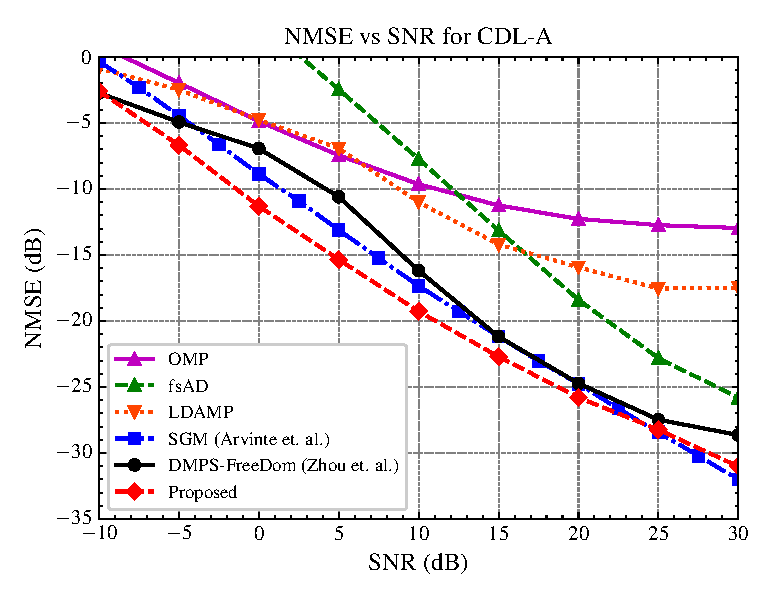
\includegraphics[width=0.48\textwidth]{images/results_CDL-A.eps}%
\label{fig:cdl-a}}
\subfigure[CDL-B]{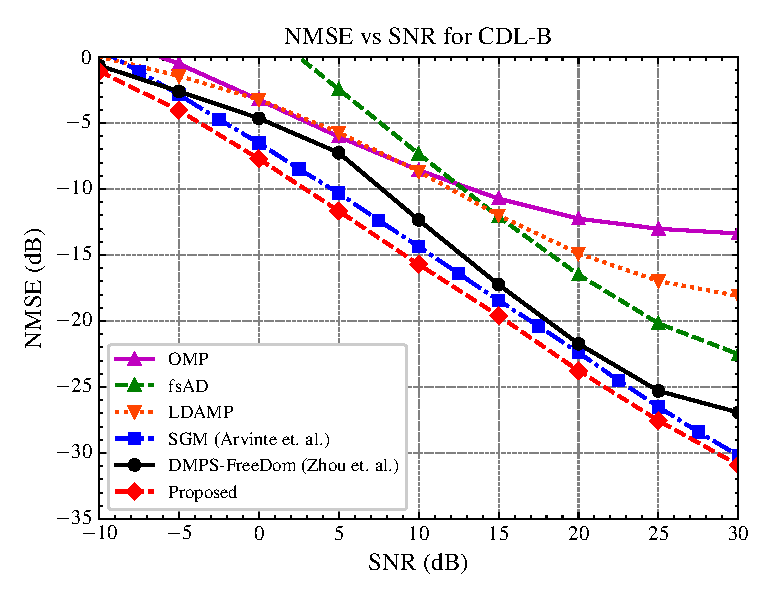
\includegraphics[width=0.48\textwidth]{images/results_CDL-B.eps}%
\label{fig:cdl-b}}
\hfil
\subfigure[CDL-C]{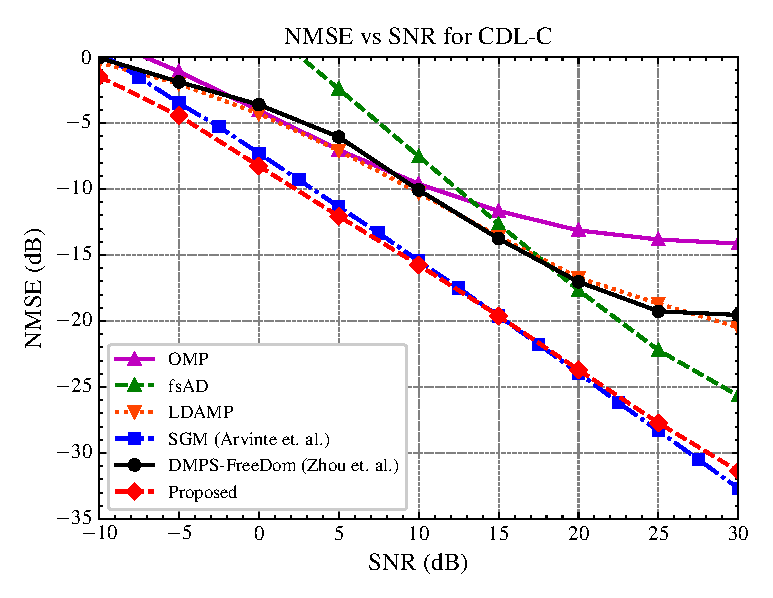
\includegraphics[width=0.48\textwidth]{images/results_CDL-C.eps}%
\label{fig:cdl-c}}
\subfigure[CDL-D]{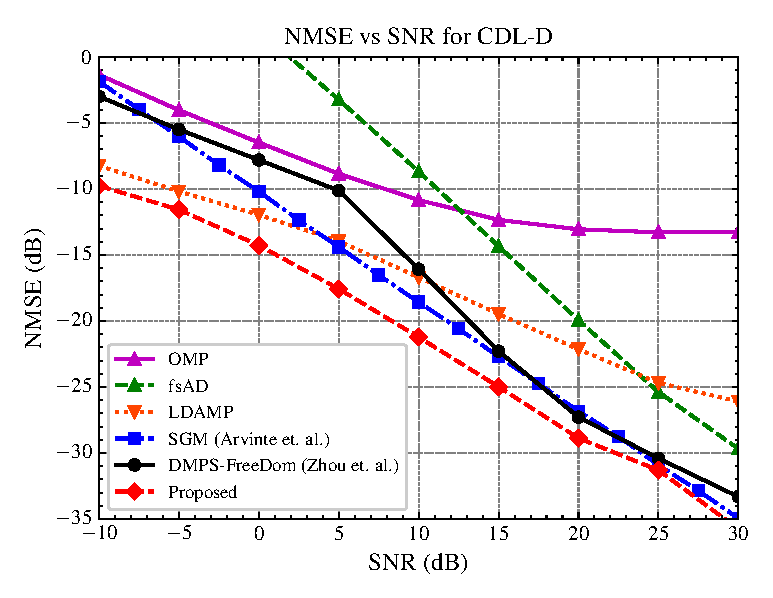
\includegraphics[width=0.48\textwidth]{images/results_CDL-D.eps}%
\label{fig:cdl-d}}
\caption{Channel estimation performance in terms of NMSE with $\rho$=0.6 (a) CDL-A. (b) CDL-B. (c) CDL-C. (d) CDL-D.}
\label{fig_sim}
\end{figure*}

\section{Conclusion}


In this letter, the novel channel estimation algorithm has been proposed to handle the accuracy, pilot overhead, and complexity simultaneously.


\bibliographystyle{IEEEtran}
% \bibliography{bib/IEEEabrv,bib/references}
\bibliography{bib/references}
\end{document}

